\documentclass{article}
\usepackage{fontspec}
\setmainfont{texgyrepagella}[Extension=.otf,UprightFont=*-regular,BoldFont=*-bold,ItalicFont=*-italic,BoldItalicFont=*-bolditalic]
\newfontfamily\blockfont{texgyreheroscn}[Extension=.otf,UprightFont=*-regular,BoldFont=*-bold,ItalicFont=*-italic,BoldItalicFont=*-bolditalic]
\usepackage{xcolor}
\usepackage{tikz}
\usetikzlibrary{arrows.meta}
\def\pages{608}
\def\spine{1.3692}
\def\bleed{0.125}
\def\trimw{7}
\def\trimh{10}
\pgfmathsetmacro{\fullw}{2*\bleed+2*\trimw+\spine}
\pgfmathsetmacro{\fullh}{2*\bleed+\trimh}
\pgfmathsetmacro{\spineL}{\bleed+\trimw}
\pgfmathsetmacro{\spineR}{\spineL+\spine}
\pgfmathsetmacro{\spineC}{\spineL+\spine/2}
\pgfmathsetmacro{\frontC}{\spineR+\trimw/2}
\pgfmathsetmacro{\backC}{\bleed+\trimw/2}
\pgfmathsetmacro{\frontw}{\fullw-\spineR}
\usepackage[paperwidth=15.6192in,paperheight=10.2500in,margin=0in]{geometry}
\pagestyle{empty}
\hyphenpenalty=10000 \exhyphenpenalty=10000
\definecolor{crimson}{HTML}{BE2742}
\definecolor{deep}{HTML}{8A1530}
\definecolor{maroon}{HTML}{39050F}
\definecolor{gold}{HTML}{D9B866}
\definecolor{cream}{HTML}{F6EEDC}
\begin{document}
\noindent
\begin{tikzpicture}[x=1in,y=1in,remember picture,overlay,shift={(current page.south west)}]
\fill[crimson] (0,0) rectangle (\fullw,\fullh);
\shade[top color=deep,bottom color=maroon!80!deep] (\spineL,0) rectangle (\spineR,\fullh);
% front
\shade[top color=deep,bottom color=maroon] (\spineR,0) rectangle (\fullw,2.2);
\node[text=white,font=\blockfont\bfseries\fontsize{70}{74}\selectfont] at (\frontC,\fullh-1.3) {\resizebox{6.15in}{!}{Bayesian Causality}};
\node[text=white,font=\blockfont\fontsize{21}{27}\selectfont,align=center] at (\frontC,\fullh-2.36)
  {Models, Accounting and the Bayesian\\Alternative to Double Machine Learning};
% the painting keeps its proportions (1838 x 1305 px): full bleed width, height from the aspect ratio
\node[anchor=south west,inner sep=0] at (\spineR,2.2) {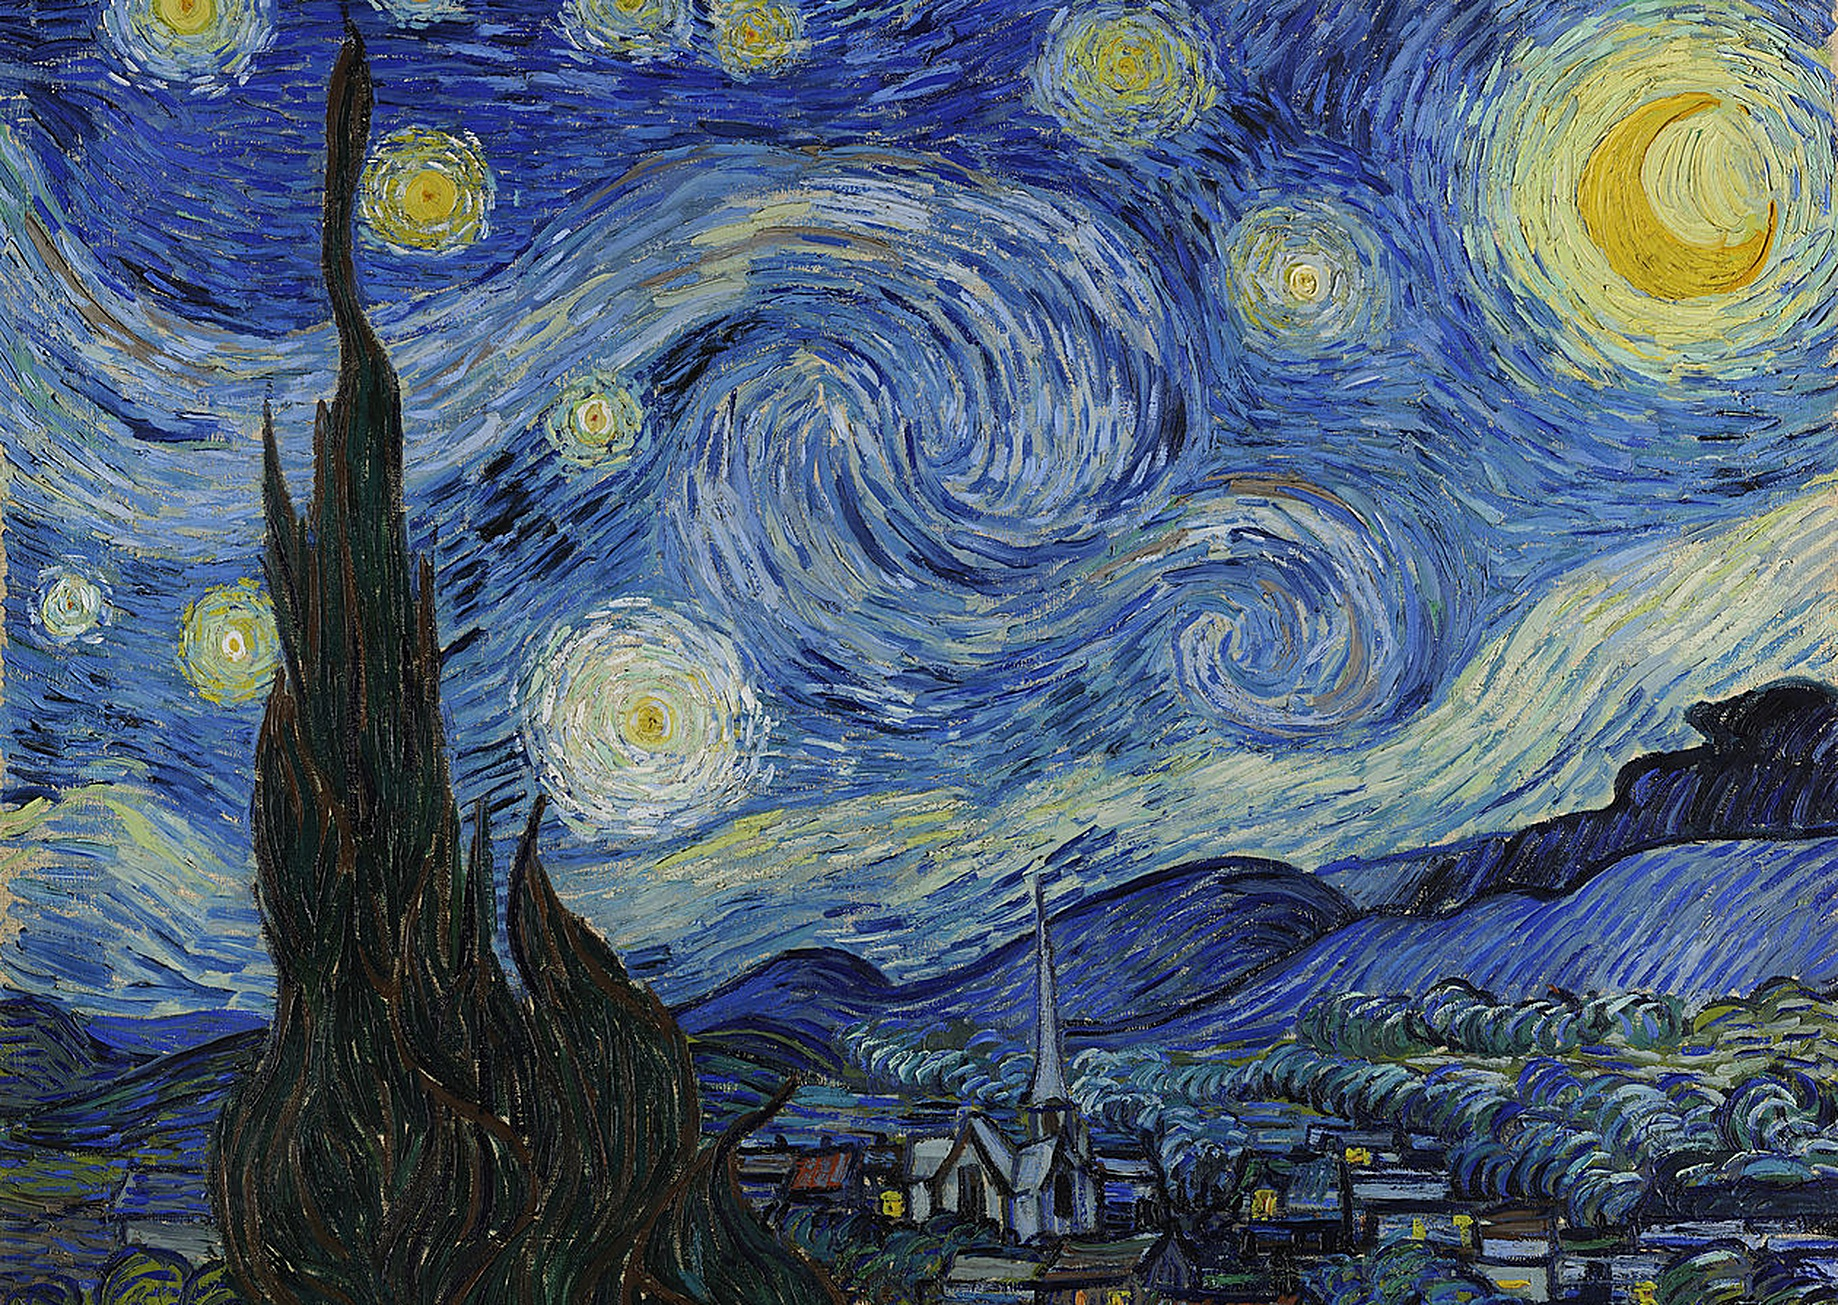
\includegraphics[width=\frontw in,keepaspectratio]{band.jpg}};
\node[text=white,font=\blockfont\bfseries\fontsize{27}{31}\selectfont] at (\frontC,1.42) {Nick Polson and Vadim Sokolov};
% spine
\node[rotate=-90,text=white,font=\blockfont\bfseries\fontsize{34}{36}\selectfont] at (\spineC,\fullh*0.6) {Bayesian Causality};
\node[rotate=-90,text=white,font=\blockfont\bfseries\fontsize{17}{19}\selectfont] at (\spineC,1.95) {Polson \;\textbullet\; Sokolov};
\draw[gold,line width=0.6pt] (\spineC-0.32,\fullh-0.75) -- (\spineC+0.32,\fullh-0.75);
\draw[gold,line width=0.6pt] (\spineC-0.32,0.6) -- (\spineC+0.32,0.6);
% back
\node[text=cream,font=\itshape\fontsize{15.5}{20}\selectfont,align=center,text width=5.6in] at (\backC,\fullh-1.0)
  {Causes and effects are discoverable,\\not by reason but by experience.};
\node[text=gold,font=\fontsize{12}{14}\selectfont] at (\backC,\fullh-1.55) {David Hume};
\draw[gold,line width=0.6pt] (\backC-1.4,\fullh-1.8) -- (\backC+1.4,\fullh-1.8);
\node[anchor=north,text=cream,font=\fontsize{12.2}{16.6}\selectfont,align=justify,text width=5.5in] at (\backC,\fullh-2.05) {%
Every causal question is a question about something we never see: the outcome that would have occurred under a different treatment. Double machine learning answers it with orthogonal scores, sample splitting and asymptotic confidence intervals. This book answers it with probability.\par\smallskip
\emph{Bayesian Causality} builds causal inference from the ground up as a problem of models and accounting. Treatment effects become posterior quantities, confounding becomes a statement about priors and likelihoods, and uncertainty is carried through every step rather than patched on at the end. Along the way the authors decompose the error of double machine learning, show where its guarantees come from and where they break, and develop Bayesian alternatives that remain coherent in finite samples, with applications from policy evaluation to the effects of mergers.\par\smallskip
Written for statisticians, economists and data scientists, and for anyone who must decide what caused what.};
\begin{scope}[shift={(\backC,3.45)},gold,line width=0.7pt]
  \node[draw,circle,minimum size=0.4in,text=cream,font=\itshape\small] (X) at (0,0.46) {X};
  \node[draw,circle,minimum size=0.4in,text=cream,font=\itshape\small] (T) at (-0.7,-0.22) {T};
  \node[draw,circle,minimum size=0.4in,text=cream,font=\itshape\small] (Y) at (0.7,-0.22) {Y};
  \draw[-{Stealth[length=5pt]}] (X) -- (T);
  \draw[-{Stealth[length=5pt]}] (X) -- (Y);
  \draw[-{Stealth[length=5pt]}] (T) -- (Y);
\end{scope}
% bios bottom left; KDP's barcode (2 x 1.2 in) goes bottom right of the back, kept clear
\node[anchor=north west,text=cream,font=\fontsize{10.3}{13.4}\selectfont,align=left,text width=3.55in] at (\bleed+0.6,2.4) {%
{\blockfont\bfseries\color{white}Nick Polson} is the Robert Law Jr.\ Professor of Econometrics and Statistics at the Booth School of Business, University of Chicago.\par\smallskip
{\blockfont\bfseries\color{white}Vadim Sokolov} is an Associate Professor in Systems Engineering and Operations Research at George Mason University, working on Bayesian methods and machine learning.\par\medskip
{\color{gold}\itshape\fontsize{9}{11}\selectfont Cover: Vincent van Gogh, \emph{The Starry Night}, 1889.\\The forces are invisible; we see only the swirl they leave.}};
% \draw[cream,dashed] (\spineL-0.25-2,\bleed+0.25) rectangle (\spineL-0.25,\bleed+0.25+1.2);
\end{tikzpicture}
\end{document}
